Transferring the knowledge between different image databases is a very popular topic in recent years due to the fast growing vision-based applications. There are many existing models to distinguish various objects. Exploiting the knowledge of these models properly can greatly help us to solve a specific recognition task.
Recently, some works have been been proposed within a framework called Hypothesis Transfer Learning (HTL) \cite{tommasi2014learning} \cite{kuzborskij2013n} \cite{jie2011multiclass} \cite{kuzborskij2013stability}. Unlike domain adaptation methods, HTL assumes only source models (called hypothesis) trained on source task can be utilized and there is no access to the data of source domain, nor any knowledge about the relatedness of the source and target distributions. 
Previous works of HTL focus on how to add a new category model to the existing $N$-category models, i.e. from a $N$-category (source) task to a $(N+1)$ (target) one. 
Previous work assumes that the hypotheses of the $N$ categories are correct for the target task \cite{kuzborskij2013n}. However, for real application in HTL, since we are not able to access the source data, in order to add a new category model, we have to collect all the data of the $N+1$ categories by ourselves. Therefore, it is trivial to simply assume that the prior hypotheses is also correct for the data we collected, especially for image recognition tasks. For example, the source hypothesis is trained from to distinguish apple and orange using the images that are bright and have high contrast level, but the images of orange and apple collected by us could be low contrast and taken in a dark environment. Therefore, the source hypothesis may fail for the same target task.
Therefore, we extend previous works by assuming that the hypotheses from source task may fail to classify the same category. 
When the source hypotheses fail, transferring from them could lead to negative transfer. 

In transfer learning, when the data distribution of the source and target domain are different, transferring the knowledge between them could even degrade the performance of the classifier on target task, which is referred to as negative transfer. On the other hand, when the data distribution are similar for the two tasks, leveraging the knowledge from source task can improve the performance of the classifier for the target one(positive transfer).
In our case, we are more likely to suffer from negative transfer due to the mismatched data distribution which could result from both the $N$ original categories and the new added category (see Figure \ref{fig:distribution}). 
How to avoid negative transfer is still an open question in transfer learning \cite{Lu201514}.
Previous works suggest that, to better utilizing the hypotheses and reduce negative transfer, decision of the algorithm should be made by combining the prior hypotheses and empirical knowledge (from the specific target task) \cite{tommasi2014learning} \cite{kuzborskij2013n} \cite{yang2007cross} \cite{aytar2011tabula}.

%\begin{figure}
%\centering
%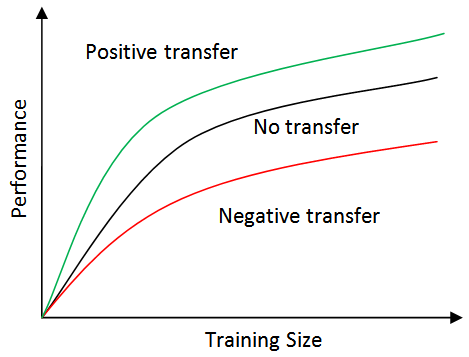
\includegraphics[scale=.5]{fig/negative.png}
%\caption{Positive transfer VS Negative transfer. %Relying on unrelated prior knowledge too much could %lead to negative transfer.}\label{fig:neg}
%\end{figure}
\begin{figure}
\centering
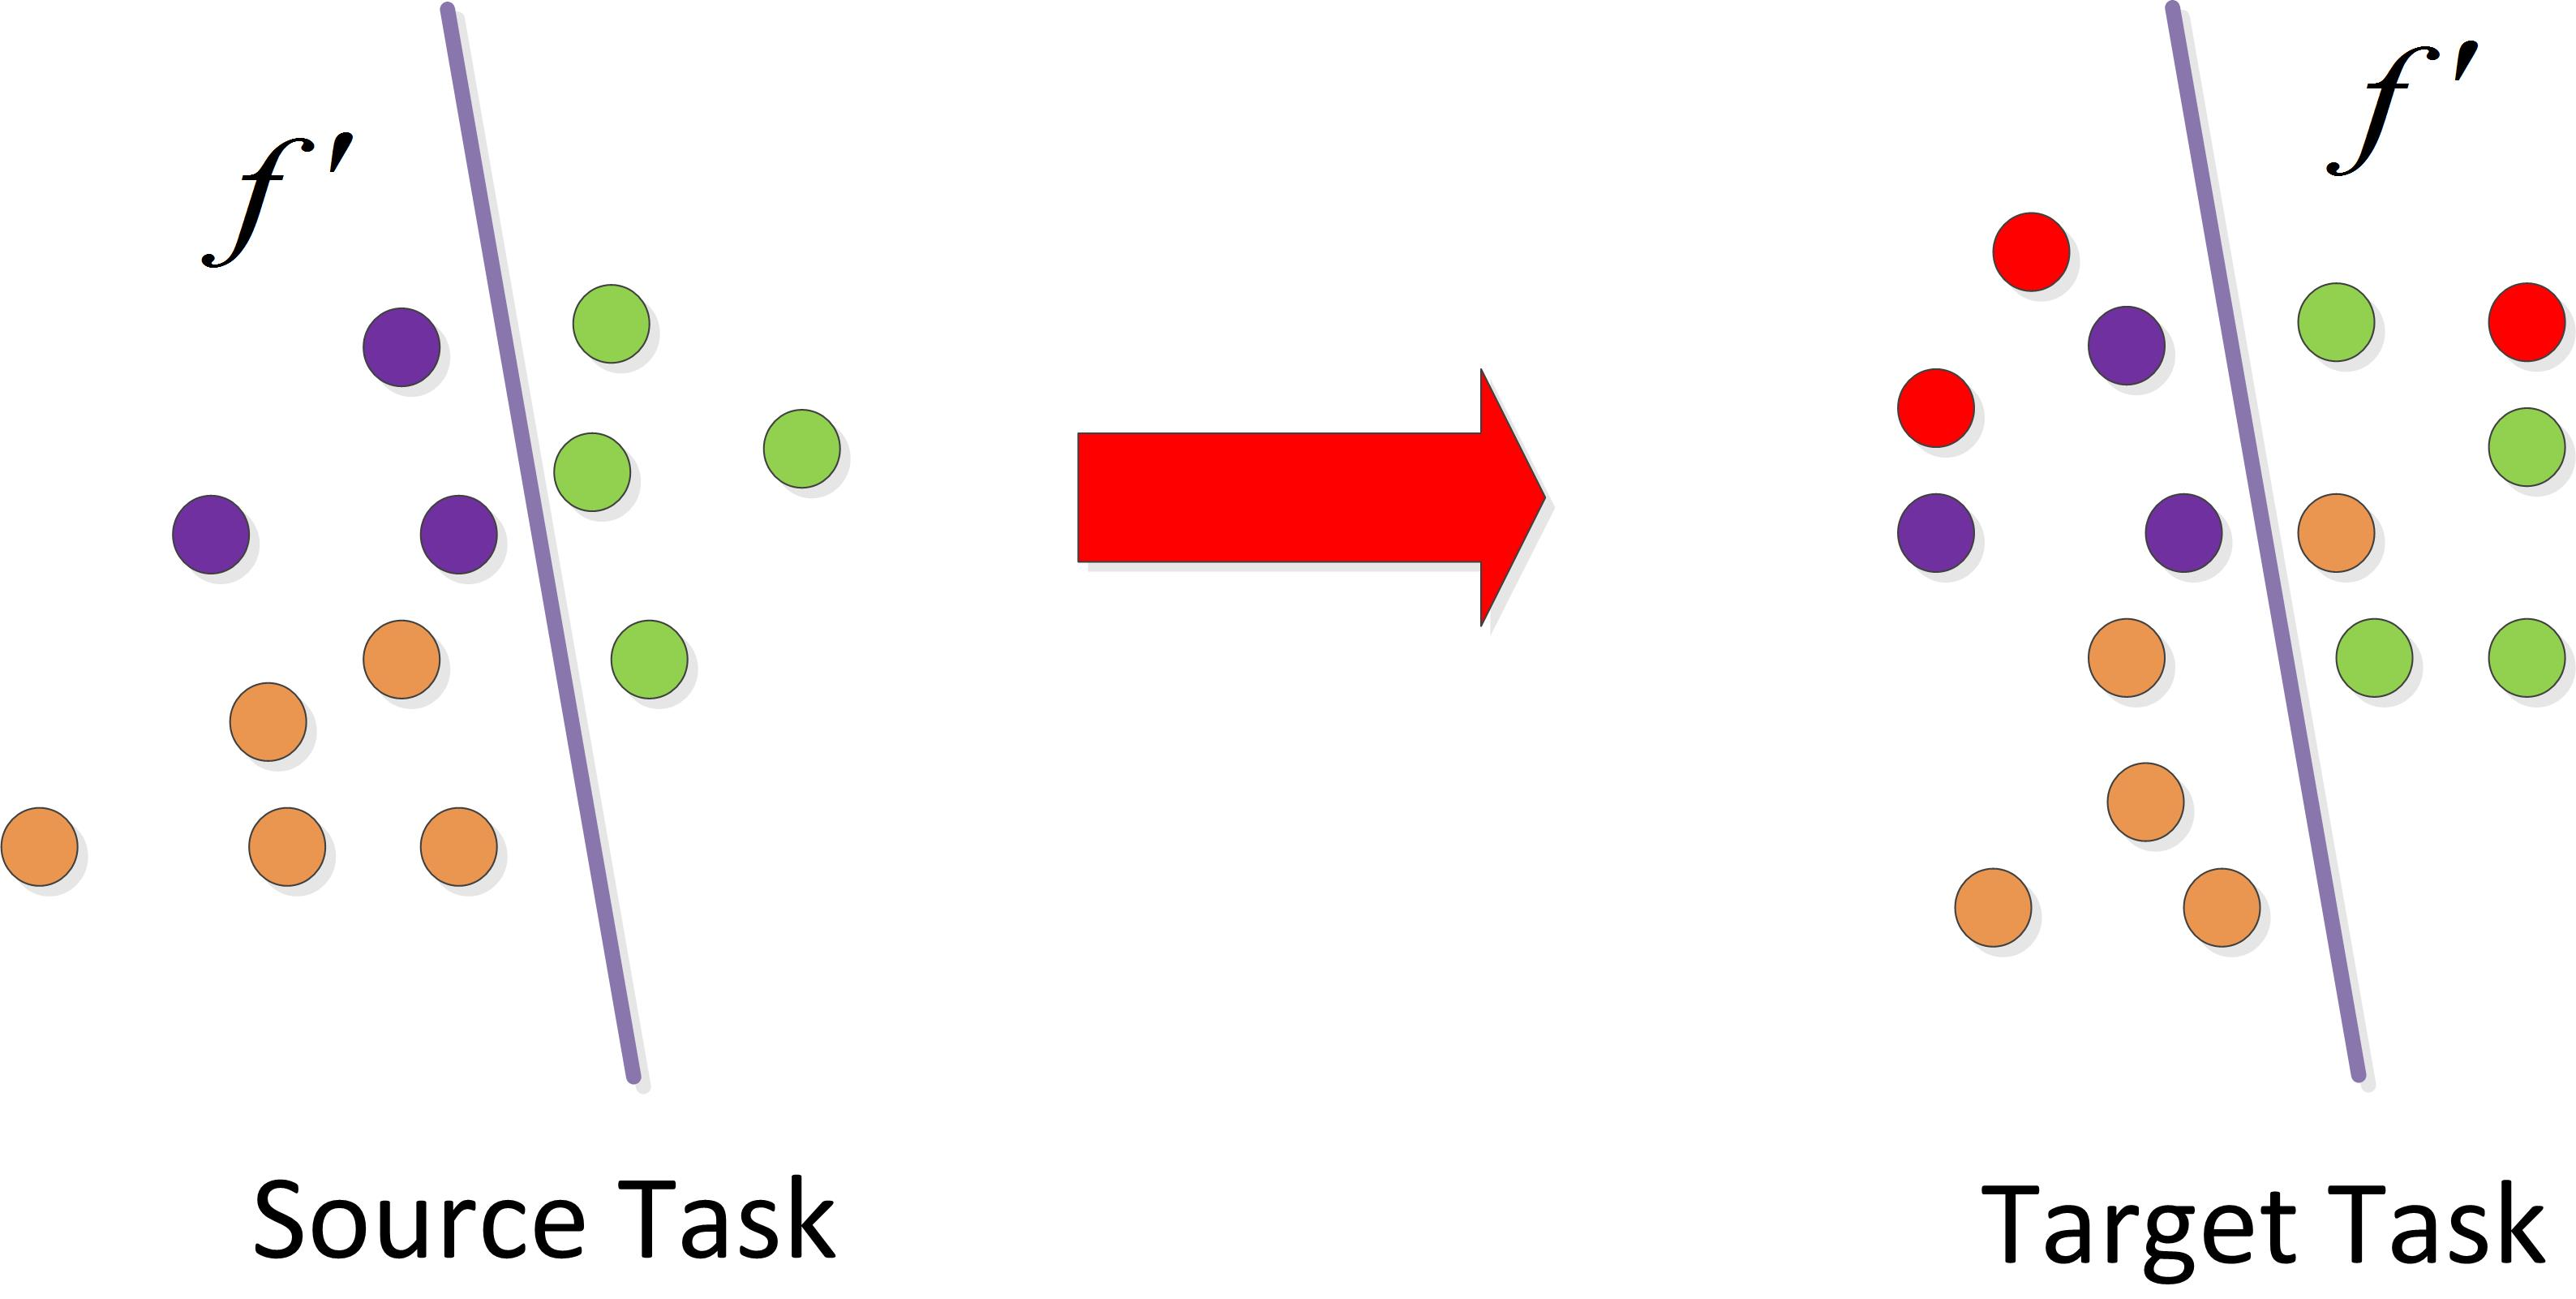
\includegraphics[scale=.4]{fig/domain.jpg}
\caption{Negative transfer happens when we transfer prior hypothesis $f'$ to target one. Points with different color represent different categories. The data distribution would change even for identical categories in different task. The new added category (red points) can also greatly affect the data distribution in target task. }\label{fig:distribution}
\end{figure}
In HTL, a number of empirical works have been attempted with Least Square Support Vector Machine (LS-SVM) \cite{kuzborskij2013stability}. 
The framework of HTL with LS-SVM has two major phrases: (I) Building binary One-Versus-All SVMs with some biased regularization. (II) Estimating transfer parameters with some objective functions.
Following these two phrases, we propose our method, called Safety Multiclass Incremental Transfer Learning (SMITLe), that can both avoid negative transfer and leverage correct hypothesis. In Phrase I, a regularization term adopted from Multi-KT \cite{tommasi2014learning} is used to adapt the $N$ original categories and the new category. As a result, the decision of each binary LS-SVM is the linear combination of the prior hypotheses and empirical knowledge controlled by some transfer parameters. In Phrase II, to measure the transferability of each prior hypothesis, we estimate our transfer parameters using multi-class prediction error based on closed-form leave-one-out (LOO) error for model evaluation.
Then we propose our novel objective function that can balance the weight between the prior hypotheses and empirical knowledge from target task. Experimental results show that SMITLe can achieve better accuracy than other baselines.

The main contributions of this paper include: (1) We propose a novel algorithm SMITLe within the HTL framework that can autonomously utilize the prior hypotheses to prevent negative transfer. (2) We also show that SMITLe can obtain the optimal solution at the rate of $O(\frac{\log(t)}{t})$ where $t$ is training iteration.

The rest of this paper is organized as follow.
In Section \ref{sec:prob}, we introduce the biased regularization terms of our problem for phrase 1 of HTL. Then, we propose a novel objective function for transfer parameter estimation, called SMITLe in Section \ref{sec:smitle}. We show that the estimated transfer parameter can distinguish the utility of the prior hypothesis and avoid negative transfer autonomously. In Section \ref{sec:exp}, we show the performance comparison between SMITLe and other baselines on a variety of experiments on AwA and Caltech datasets in three different scenarios.
